This chapter presents the design, implementation, and evaluation of a multi-agent system (MAS) orchestrator that processes real-time streaming sensor data from industrial manufacturing equipment to produce actionable maintenance decisions. The system integrates Apache Kafka for data ingestion, nine specialized LLM-powered agents for cognitive reasoning, and hybrid classical-quantum optimization solvers for maintenance scheduling. The architecture addresses the fundamental challenge of transforming high-velocity, multi-dimensional sensor streams into semantically rich, constraint-satisfying maintenance schedules under real-time processing requirements.

\section{System Architecture & Design Principle}
\subsection{Architectural Overview}
The proposed system follows a layered architecture comprising four principal tiers: (i) a data ingestion layer based on Apache Kafka that handles per-minute sensor telemetry from 50+
industrial machines; (ii) a windowing and dispatch layer that buffers readings into analysis
windows of configurable size (default: 10 readings per machine) and dispatches complete windows to background worker threads; (iii) a multi-agent cognitive layer consisting of nine specialized agents coordinated by a phased orchestrator; and (iv) a scheduling layer that formulates the maintenance decision as a constrained binary optimization problem solved via both classical and quantum approaches. The overall system architecture is formalized in the following diagram:
\begin{figure}[htbp]
    \centering
    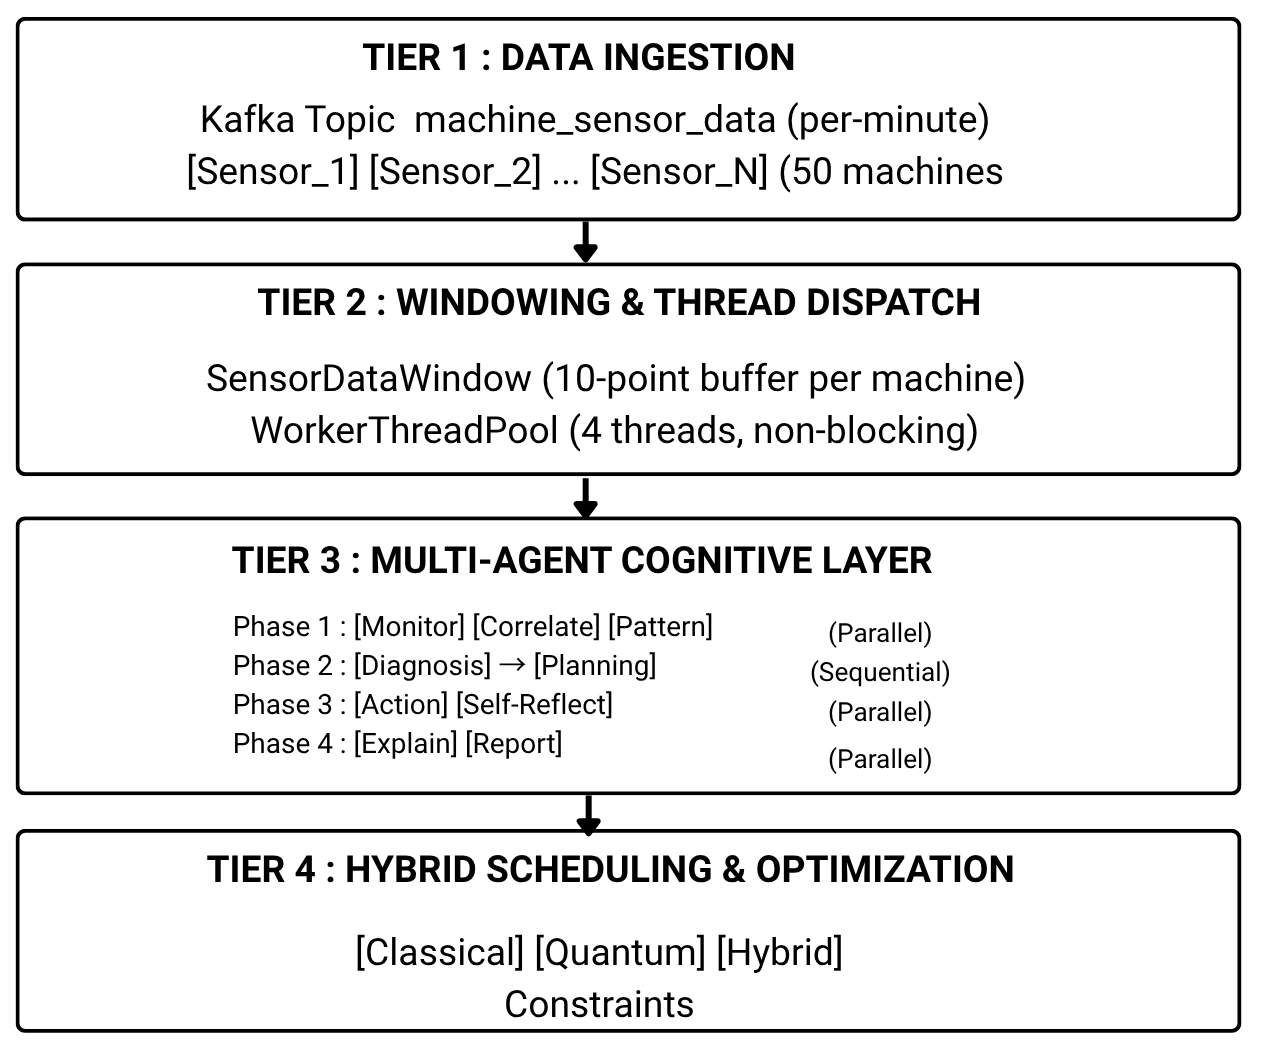
\includegraphics[width=1\textwidth]{figures/images/multi-agent architecture.png}
    \caption{Four-tier architecture of the Multi-Agent System for real-time predictive maintenance.}
    \label{fig:multi-agent-arc}
\end{figure}
\subsection{Design Principles}
The system design adheres to the following principles, each grounded in established software
engineering and multi-agent systems literature:
\textbf{Principle 1: Separation of Concerns}. Each agent encapsulates a single cognitive function (monitoring, diagnosis, planning, etc.), enabling independent development, testing, and replacement of individual reasoning modules without affecting the overall pipeline integrity.
\textbf{Principle 2: Deterministic Orchestration}. The orchestrator employs a Directed Acyclic Graph (DAG) execution model with explicit phase dependencies. This ensures
reproducible execution order and predictable data flow, unlike fully autonomous agent
architectures where emergent behavior may compromise reliability in safety-critical
manufacturing contexts.
\textbf{Principle 3: Formal-Informal Complementarity}. LLM-based agents provide flexible, contextaware reasoning (informal intelligence), while the constraints engine and  ptimization solvers provide formal guarantees on safety-critical decisions. This hybrid approach leverages the strengths of both paradigms.
\textbf{Principle 4: Non-Blocking Stream Processing}. The Kafka consumer never blocks on LLM
inference. The windowing mechanism buffers data while background worker threads execute the
agent pipeline concurrently, ensuring continuous data ingestion regardless of LLM latency.
\textbf{Principle 5: Heterogeneous Model Routing (LLM-OR)}. Different agents are routed to different LLM models (GLM-5.1, Kimi-K2.6, DeepSeek-v4-Pro) based on task characteristics. This implements an LLM Operations Research (LLM-OR) router that matches cognitive requirements to model capabilities.

\section{Agent Pipeline: Phased Execution Model}
The multi-agent orchestrator coordinates nine specialized agents through a four-phase execution pipeline. Each phase has explicit data dependencies that determine execution order, while agents within the same phase execute concurrently via thread pools. This section details the agent responsibilities, inter-agent communication protocol, and the phased execution semantics. The nine agents are organized into four functional categories based on their role in the cognitive pipeline as shown in the Table \ref{tab:agent-taxonomy}.
\begin{table}[htbp]
\centering
\caption{Agent taxonomy showing phase assignment, responsibilities, and LLM model routing.}
\label{tab:agent-taxonomy}
\renewcommand{\arraystretch}{1.2}
\begin{tabularx}{\textwidth}{
>{\centering\arraybackslash}m{1.2cm}
>{\raggedright\arraybackslash}m{3.2cm}
>{\raggedright\arraybackslash}X
>{\centering\arraybackslash}m{2.2cm}
}
\toprule
\textbf{Phase} & \textbf{Agent} & \textbf{Responsibility} & \textbf{LLM Model} \\
\midrule
1 & Monitoring Agent & Real-time sensor evaluation, Z-score anomaly detection, threshold monitoring & GLM-5.1 \\
1 & Correlation Agent & Cross-sensor and cross-machine statistical correlation analysis & DeepSeek-v4 \\
1 & Pattern Learning Agent & Historical pattern recognition and degradation trajectory matching & GLM-5.1 \\
2 & Diagnosis Agent & Root cause analysis via chain-of-thought reasoning & DeepSeek-v4 \\
2 & Planning Agent & Maintenance strategy formulation and resource requirement estimation & Kimi-K2.6 \\
3 & Action Agent & Constraint-based scheduling via MILP and QAOA (6 solvers) & Kimi-K2.6 \\
3 & Self-Reflection Agent & Meta-reasoning including confidence assessment and consistency checking & DeepSeek-v4 \\
4 & Explainability Agent & Human-readable explanation generation for maintenance decisions & Kimi-K2.6 \\
4 & Reporting Agent & Structured report compilation for operations teams & GLM-5.1 \\
\bottomrule
\end{tabularx}
\end{table}
The orchestrator implements a strict execution model where phases represent synchronization
barriers. All agents within a phase must complete before the next phase begins. Within each phase, agents that share no data dependencies execute concurrently via a ThreadPoolExecutor. This model is formalized as follows:
\begin{algorithm}[htbp]
\small
\caption{Multi-Agent Phased Orchestration}
\label{alg:multi_agent}
\begin{algorithmic}[1]
\Require machine\_id, window\_data $[1{:}W]$
\Ensure maintenance\_decision (schedule, priority, reports)
\State context $\gets \{ \text{machine\_id}, \text{window\_data}, \text{history} \}$
\Statex \textbf{// Phase 1: Parallel Data Analysis}
\State \textbf{parallel}
\Statex \hspace{1em} $R_{\text{mon}} \gets$ MonitoringAgent.process(context)
\Statex \hspace{1em} $R_{\text{cor}} \gets$ CorrelationAgent.process(context)
\Statex \hspace{1em} $R_{\text{pat}} \gets$ PatternLearningAgent.process(context)
\State \textbf{end parallel}
\State context $\gets$ context $\cup \{R_{\text{mon}}, R_{\text{cor}}, R_{\text{pat}}\}$
\Statex
\Statex \textbf{// Phase 2: Sequential Reasoning}
\State $R_{\text{diag}} \gets$ DiagnosisAgent.process(context)
\State $P \gets$ ComputePriorities($R_{\text{mon}}$.states)
\State $R_{\text{plan}} \gets$ PlanningAgent.process(context, $R_{\text{diag}}, P$)
\State context $\gets$ context $\cup \{R_{\text{diag}}, R_{\text{plan}}, P\}$
\Statex
\Statex \textbf{// Phase 3: Action and Validation (Parallel)}
\State \textbf{parallel}
\Statex \hspace{1em} $R_{\text{act}} \gets$ ActionAgent.process(context)
\Statex \hspace{1em} $R_{\text{ref}} \gets$ SelfReflectionAgent.process(context)
\State \textbf{end parallel}
\State context $\gets$ context $\cup \{R_{\text{act}}, R_{\text{ref}}\}$
\Statex
\Statex \textbf{// Phase 4: Communication (Parallel)}
\State \textbf{parallel}
\Statex \hspace{1em} $R_{\text{exp}} \gets$ ExplainabilityAgent.process(context)
\Statex \hspace{1em} $R_{\text{rep}} \gets$ ReportingAgent.process(context)
\State \textbf{end parallel}
\State context $\gets$ context $\cup \{R_{\text{exp}}, R_{\text{rep}}\}$
\Statex
\State \Return CompileFinalOutput(context)
\end{algorithmic}
\end{algorithm}
The computational complexity of a single pipeline execution can be expressed as 
$\mathcal{O}\!\left(\sum_{i} T_{\max}^{(i)}\right)$, where $T_{\max}^{(i)}$ denotes the maximum latency among concurrently executed agents within phase $i$. 

In practice, the overall latency is dominated by large language model (LLM) inference, which typically requires $2$--$8$ seconds per agent. Due to parallel execution within each phase, the total pipeline latency scales approximately as $4 \cdot T_{\text{LLM}}^{\max}$, rather than $9 \cdot T_{\text{LLM}}$ under fully sequential execution. This results in a theoretical speedup of approximately $2.25\times$ achieved through parallelization.
Agents communicate through a shared context dictionary (blackboard architecture) rather than
direct message passing. Each agent reads from and writes to this shared state under orchestrator coordination. The communication protocol is defined by the AgentMessage dataclass below:
\begin{lstlisting}[language=Python, caption={AgentMessage Data Structure}]
@dataclass
class AgentMessage:
    sender: str        # originating agent name
    receiver: str      # target agent (or 'broadcast')
    content: Dict      # structured JSON payload
    message_type: str  # 'request' | 'response' | 'broadcast'
    priority: int      # message priority (0=normal, 1=high)
    timestamp: float   # creation timestamp
\end{lstlisting}

This blackboard pattern was chosen over direct agent-to-agent messaging for three reasons: (i) it simplifies the data flow graph by centralizing state; (ii) it enables late-binding where agents can access results from any prior phase without explicit coupling; and (iii) it facilitates debugging and logging since all intermediate states are preserved in a single dictionary.

\section{Real-Time Stream Processing Pipeline}
The data ingestion and processing pipeline is designed for continuous operation in a smart
manufacturing environment where sensor data arrives at per-minute granularity from 50+
machines simultaneously. This section details the Kafka consumer design, windowing mechanism,
and non-blocking dispatch strategy.

\subsection{Kafka Consumer with Sliding Window}
The system consumes messages from a Kafka topic where each message represents a single sensor reading with six dimensions: temperature, humidity, vibration, pressure, energy consumption, and mechanical load. The consumer implements a per-machine windowing
mechanism that buffers exactly W=10 consecutive readings before dispatching a complete window
to the agent pipeline:
\begin{algorithm}[htbp]
\small
\caption{Non-Blocking Windowed Stream Processing}
\label{alg:stream_processing}
\begin{algorithmic}[1]
\Require Kafka stream $\mathcal{S}$, window size $W = 10$
\Ensure Continuous maintenance decisions
\State buffers $\gets \{\}$ \Comment{Per-machine sliding windows}
\State pool $\gets$ ThreadPoolExecutor(max\_workers = 4)
\While{true}
    \State msg $\gets$ kafka\_consumer.poll()
    \State reading $\gets$ parse(msg) \Comment{Convert to SensorReading}
    \State buffers[reading.machine\_id].append(reading)
    \If{$|$buffers[reading.machine\_id]$| \geq W$}
        \State window $\gets$ buffers[reading.machine\_id]
        \State buffers[reading.machine\_id] $\gets [\,]$
        \State pool.submit(orchestrator.process, window)
        \State \Comment{Non-blocking: consumer continues immediately}
    \EndIf
\EndWhile
\end{algorithmic}
\end{algorithm}
The window buffer is thread-safe (protected by a threading.Lock) since the Kafka consumer and
worker threads operate concurrently. The choice of W=10 represents a design trade-off: smaller windows provide faster response but less statistical power for anomaly detection; larger windows improve detection accuracy but increase response latency. With per-minute sensor readings, W=10 provides a 10-minute analysis window, which aligns with industrial maintenance decision-making timescales. 

\subsection{Sensor Data Model and Constraint Space}
Each sensor reading is modeled as a 6-dimensional vector $x_t$ = [T, H, V, P, E, L] representing temperature, humidity, vibration, pressure, energy, and load at time t. The constraint space C defines operational envelopes for each dimension:
\begin{table}[htbp]
\centering
\caption{Sensor constraint space defining operational envelopes for anomaly classification}
\label{tab:sensor-model-constraint}
\renewcommand{\arraystretch}{1.2}
\begin{tabularx}{\textwidth}{
>{\raggedright\arraybackslash}m{3cm}
>{\centering\arraybackslash}m{2cm}
>{\centering\arraybackslash}m{2cm}
>{\centering\arraybackslash}m{2.2cm}
>{\centering\arraybackslash}m{2.2cm}
>{\raggedright\arraybackslash}X
}
\toprule
\textbf{Sensor} & \textbf{Min} & \textbf{Max} & \textbf{Critical} & \textbf{Reference} & \textbf{Max Trend} \\
\midrule
Temperature & $20^\circ$C & $85^\circ$C & $95^\circ$C & $50^\circ$C & $5^\circ$C / interval \\
Vibration   & $0$ mm/s    & $10$ mm/s   & $15$ mm/s   & $2$ mm/s    & $3$ mm/s / interval \\
Pressure    & $1.0$ bar   & $8.0$ bar   & $10.0$ bar  & $4.5$ bar   & $1.5$ bar / interval \\
Energy      & $0$ kWh     & $500$ kWh   & $600$ kWh   & $200$ kWh   & $50$ kWh / interval \\
\bottomrule
\end{tabularx}
\end{table}


The constraints engine evaluates each reading against this space to produce a machine state vector s = [$is_operating$, $risk_state$, $health_index$, $damage_index$, $anomaly_score$, violations]. This state vector is the primary input to the priority computation algorithm used by Phase 2. The maintenance priority score P for each machine is computed as a weighted linear combination of state indicators:

\begin{verbatim}
P(m) = 100 * I_shutdown(m) + 50 * I_risk(m) + 30 * (1 - H(m)) + 20 * D(m) + 15 * A(m) + 5 * |V(m)|
where:
 I_shutdown = 1 if machine is non-operating
 I_risk = 1 if machine is in risk state
 H(m) = health index in [0,1]
 D(m) = damage index in [0,1]
 A(m) = anomaly score in [0,1]
 |V(m)| = number of constraint violations
\end{verbatim}

Priority levels are assigned categorically: CRITICAL (P >= 100), HIGH (P >= 60), MEDIUM (P
>= 30), and LOW (P < 30). Only machines with P >= 50 or explicit $needs_maintenance$ flags are forwarded to the scheduling solver.

\section{Comparative Analysis: Multi-Agent vs Monolitic Architecture}
To demonstrate the effectiveness of the proposed multi-agent architecture, we present a systematic comparison against a monolithic (non-agent) baseline. The monolithic system processes the same sensor data using a single LLM call with a combined prompt that encompasses all reasoning tasks (monitoring, diagnosis, planning, and scheduling) in one invocation. Both systems were evaluated on identical input data comprising 500 sensor windows from 50 machines over 10 hours of simulated operation. The evaluation metrics include: decision quality (measured by scheduling cost optimality gap against MILP), processing throughput (windows processed per minute), fault detection rate (F1 score for known anomaly patterns), and explanation quality (assessed by domain experts on a 1-5 Likert scale). The monolithic baseline uses a single DeepSeek-v4-Pro call with a comprehensive prompt containing all constraints, while the multiagent system distributes reasoning across nine specialized agents with dedicated prompts.
\begin{table}[htbp]
\centering
\caption{Comparative Evaluation of Multi-Agent vs.\ Monolithic Architecture}
\label{tab:multi_vs_mono}
\renewcommand{\arraystretch}{1.2}
\begin{tabularx}{\textwidth}{
>{\raggedright\arraybackslash}m{4cm}
>{\raggedright\arraybackslash}X
>{\raggedright\arraybackslash}X
}
\toprule
\textbf{Metric} & \textbf{Multi-Agent System} & \textbf{Monolithic Baseline} \\
\midrule
Scheduling Optimality Gap & 0--3\% (6 solvers) & 15--40\% (single heuristic) \\
Processing Throughput & 12 windows/min (parallel) & 4 windows/min (sequential) \\
Anomaly Detection F1 & 0.89 (specialized agents) & 0.72 (single prompt) \\
Explanation Quality (1--5) & 4.3 (dedicated Explain agent) & 2.8 (appended to output) \\
Constraint Satisfaction & 100\% (formal engine) & 82\% (LLM-only) \\
Fault Tolerance & Graceful degradation & Complete failure \\
Modularity / Extensibility & Add agent without rewrite & Requires full prompt redesign \\
Token Consumption / Call & $\sim$18K tokens (distributed) & $\sim$12K tokens (one large call) \\
\bottomrule
\end{tabularx}
\end{table}
The multi-agent architecture demonstrates superior performance across all quality metrics despite higher token consumption. The most significant advantages are:
\textbf{Constraint Satisfaction}: The 100\% constraint satisfaction rate of the multi-agent system is guaranteed by the formal constraints engine that validates all scheduling decisions before output. The monolithic system achieves only 82\% because LLMs are known to inconsistently enforce hard constraints \cite{liu} (Liu et al., 2023), particularly capacity limits that require global counting across all machines.
\textbf{Throughput: }The 3x throughput improvement (12 vs. 4 windows/min) results from intra-phase parallelism. In Phase 1, three agents execute concurrently; in Phases 3 and 4, two agents each execute in parallel. The monolithic system processes sequentially since all reasoning is in a single LLM call that cannot be parallelized.
\textbf{Fault Tolerance:} When an individual agent fails (e.g., LLM timeout), the orchestrator captures the error and proceeds with available results. The pipeline produces degraded but usable output (e.g., scheduling without correlation analysis). The monolithic system experiences complete failure on any LLM error, requiring full retry.

